%!TEX root = /home/glauffer/Dropbox/FURG/final_project/monografia/monografia.tex
\chapter{Metodologia}
\label{cap:tecnicas}
%\textcolor{red}{descrição das técnicas em detalhes}

Neste capítulo será abordado o método utilizado para a determinação de períodos de estrelas variáveis pulsantes, assim como a metodologia aplicada para a análise do método e criação do algoritmo, cobrindo o catálogo utilizado para obtenção dos dados e o formato dos mesmos.

%A busca por periodicidades na curva de luz de uma estrela variável é um dos mais importantes processos na análise de dados observacionais. A importância desse processo é devido as grandezas físicas que podemos derivar a partir do período. Dentro dessas grandezas, a distância é sem duvidas uma das mais importantes pois, a determinação de distâncias astronômicas é um dos problemas fundamentais da astronomia.

%Devido a importância na determinação de períodos, diversos métodos surgiram ao longo dos anos. Uma técnica comum para demonstrar os períodos em um dado seria o \textit{Periodograma} ou \textit{Espectro de Potência}. Neste método, a intensidade do sinal gerado através dos dados é mostrado em um gráfico versus o período. Os picos desse gráfico seriam o período principal com os seu harmônicos. Alguns desse métodos utilizam o método dos mínimos quadrados para ajustar uma função com período conhecido à curva de luz da estrela \citep{lomb}. Outros determinam o período através dos picos no espectro de Fourier \citep{mello81} ou fazem analise de variância nesses picos \citep{aov}. Ou também, calculam a minimização da dispersão dos pontos observacionais no espaço de fase \citep{Cincotta1999, entropy, ce}.

%Um dos principais problemas na determinação de períodos está nos dados observacionais. Dados que contenham uma semana de observação são impróprios para objetos que possuem período na ordem de anos. Para calcularmos o período com confiança, precisamos que o tempo de observação seja de pelo menos o dobro do tempo do período, de acordo com o \textit{Teorema de Nyquist}. Se esta condição não é satisfeita, podemos obter mais de um período ou o período errado para o nosso dado (este efeito é conhecido como \textit{Aliasing}). Outro motivo de erro nos dados são os espaçamentos entre as observações. Devido a estes espaçamento, as técnicas de detecção de períodos podem identificar períodos que aparentemente produzem uma curva de luz adequada mas que não são os períodos corretos, sendo uma fonte de Aliasing. Alguns motivos para espaçamento entre os dados são a disponibilidade do telescópio, a limitação de observação para o turno da noite e a posição da lua nos telescópios terrestres, o que pode fazer com que as observações sejam espaçadas por até um mês. Por estes motivos apresentados, seria interessante aprimorar técnicas que sejam independentes deste espaçamento entre os dados, como as técnicas que utilizam a dispersão da curva de luz no espaço de fase, técnica utilizado pelo método aplicado neste trabalho.


%\begin{comment}
%
%\section{Principais Técnicas de Observação}
%
%O primeiro dispositivo utilizado na observação de estrelas variáveis foi o olho humano.
%Embora este dispositivo nos seja muito útil no dia a dia, para a observações de estrelas não seria o mais adequado pois a sua precisão para captar brilho é baixa ($\approx 0.1$) o que faz com que apenas estrelas com varição de algumas unidades de magnitude nos chamaria a atenção. Também, a percepção de mudanças no céu noturno não é possível com observações feitas em telescópios. Apenas com a introdução da placas fotográficas que foi possível ter um controle mais efetivo desta variações.
%
%\subsection{Métodos fotográficos}
%
%As primeiras fotografias astronômicas foram obtidas em torno de 1850 e 1860 utilizando o Daguerreótipo (ou método de Daguerre), que consistia em fixar a imagem em uma placa de cobre com uma fina camada de prata. Devido a sua limitação para variações em luminosidade, apenas fotos da Lua, Sol e estrelas mais brilhantes foram obtidas por este método. Apenas com o advento do método de placa seca em 1871 foi possível melhorar as observações de estrelas variáveis. Porém, identificar estrelas variáveis em placas fotográficas era um trabalho tedioso. Uma única imagem do céu noturno poderia conter milhares de estrelas. Uma forma utilizada para tentar identificar a variações de brilho seria utilizar uma série de 10 ou mais fotografias da mesma porção do céu, fazer divisões nas fotografias e comparar todas elas para perceber variações nos brilhos das estrelas. Através desta técnica aplicada em clusters globulares, o astronomo Solon Bailey detectou mais de 500 variáveis \citep{Bailey1902}.
%
%Outros métodos surgiram para aprimorar a identificação da estrelas variáveis. Um desses métodos seria a sobreposição dos negativos e positivos da mesma fotografia. No positivo, as estrelas seriam brancas em um fundo escuro enquanto que no negativo seria o oposto. Se o brilho de uma estrela variasse, a imagem negativa seria menor ou maior do que a imagem positiva.
%
%Uma das principais ferramentas utilizadas para analisar as fotografias de estrelas era o dispositivo chamado \textit{Comparador Blink} (do inglês, \textit{Blink Comparator}). Neste dispositivo, duas placas fotográficas eram analisadas, uma por cada olho do observador. Se as imagens fossem iguais, não seria identificado variação, porem, alguma variação no brilho de uma imagem para a outra seria percebida pela mudança de tamanho da estrela entre as imagens.
%
%Embora a quantidade de estrelas variáveis descobertas a partir de 1880 aumentou drasticamente devido ao métodos fotográfico, esta técnica não consegue identificar pequenas variação no brilho, apenas variações em torno de um terço da magnitude máxima da estrela, fazendo com que uma parcela das estrelas não fossem identificadas. Assim, surgiu a necessidade de algum método mais efetivo.
%
%
%\subsection{Métodos fotoelétricos}
%
%O desenvolvimento da fotometria fotoelétrica ocorreu na década de 40. Estes métodos captam a luz em uma célula fotossensível que converte o fluxo de fótons recebido em sinal elétrico através do efeito fotoelétrico. Os sistemas de magnitudes (filtros) foram desenvolvidos para estes tipos de equipamentos.
%
%Os primeiros dispositivos  desta época utilizavam placas de selênio e eram capazes de captar o brilho de apenas um objeto por vez. A magnitude de uma estrela era obtido fazendo a leitura do brilho da estrela e do céu noturno a sua volta, após era feita a leitura apenas de uma porção do céu e subtraído da leitura da estrela.
%
%Uma das revoluções nesta área de observação ocorreu com a utilização das células fotomultiplicadoras na astronomia em 1936 pela Radio Corporation of America (RCA) \citep{Miles2007}. As vantagens destas células são a amplificação do sinal observado, o que melhorou a precisão das medidas, maior faixa de detecção ($640 \si{nm}$ até a faixa do vermelho) e menor ruído. Embora a célula fotomultiplicadora tenha trazido grandes avanços na astronomia observacional, esta tecnologia ainda era limitada a observar objetos individuais. A grande revolução ocorreu com a utilização dos detectores em área.
%
%\subsection{Detectores em área}
%
%Em 1969 as placas CCD (do inglês, \textit{Charged Coupled Device}) foram criadas no Bell Laboratories nos Estado Unidos. Este dispositivo apresenta alta sensibilidade espectral, podendo ser utilizado em faixas de $350 a 1000 \si{nm}$, habilidade de detectar luz em área quando dispostas em conjunto (chamado de \textit{CCD Array}) e por transformar a observação em sinal digital sendo possível analisar as imagens em computadores, facilitando o trabalho de detecção de periodicidades através dos métodos de detecção de períodos.
%
%As placas CCD são os dispositivos utilizados no grandes projetos de levantamento de dados astronômicos (\textit{Surveys}) atualmente. Um destes projetos é o OGLE que atualmente está atuando em sua quarta fase. A terceira fase \citep{Udalski2008} que já esta completa e possui os dados públicos\footnote{\url{http://ogledb.astrouw.edu.pl/~ogle/CVS/}} e parte desses dados são utilizados neste trabalho, monitorou mais de 200 milhões de estrelas nas Nuvens de Magalhães e se espera detectar em torno de um milhão de estrelas variáveis .
%
%\end{comment}

%\section{Amostragem}

%\textcolor{red}{A vantagem de utilizar as RRLyraes AB é tal que a distancia pode ser obtida pela relaçao pl e a extinção pela relacao periodo-cor \citep{Pejcha2009}}

%\textit{falar sobre a amostragem das Lyraes e Nyquist}

%\section{Analise de Fourier}

%\subsection{Lomb-Scargle}

%\begin{comment}
%
%\section{Espaço de fase}
%
%Quando uma estrela possui um comportamento periódico, a variação em sua magnitude é representada em ciclos iguais. Cada ciclo é uma fase. Se os ciclos são iguais, não importa qual ciclo nos estamos observando, apenas onde nos estamos no ciclo. Assim, o espaço de fase é uma representação de todos os ciclos observados em apenas uma fase, ou em apenas um ciclo. Assim, os pontos de sobrepõem e formam uma oscilação geral da estrela. Este espaço de fase é calculado pela seguinte expressão,
%\begin{equation}
%\phi_i = \frac{t_i}{P} - \Big[\frac{t_i}{P}\Big]
%\end{equation}
%em que $t_i$ é o i-ésimo dado do tempo, $P$ é o período de oscilação da magnitude e a quantidade entre colchetes representa apenas o numero inteiro da divisão.
%%Most of the entropy based methods are based on information entropy. In information theory, entropy is a measure of the uncertainty in a random variable. So, the entropy measures the lack of information of one variable.
%
%%Information theory based methods extract information from the probability density function and so include higher-order statistical moments present in the data whereas Fourier or analysis of variance techniques are based only on second-order statistical analyses. This implies that information theory brings better modeling of the underlying process and robustness to noise and outliers \citep{graB13}.
%
%
%%Para calcular a entropia condicional, primeiramente é necessário transformar os dados para o espa\c{c}o de fase e normalizar a luminosidade da estrela. Quando os dados são lidos pelo programa, ele gera dois vetores, um com os dados sobre o tempo e outro com os dados sobre a luminosidade da estrela. Para transformar o tempo em fase é necessário dividir cada um dos elementos do vetor tempo pelo período e subtrair o inteiro desta divisão,
%%\begin{equation}
%%\phi_i = \frac{t_i}{P} - \Big[\frac{t_i}{P}\Big]
%%\end{equation}
%%assim, temos um novo vetor com os dados da fase. O gráfico que pode ser obtido com os dados da fase e da luminosidade representa a dispersão da série temporal no espa\c{c}o de fase. A entropia condicional é calculada a partir desta dispersão.
%
%%Um exemplo de espa\c{c}o de fase é dado a seguir:
%
%
%\begin{figure}[h!]
%\centering
%\begin{subfigure}{.5\textwidth}
%  \centering
%  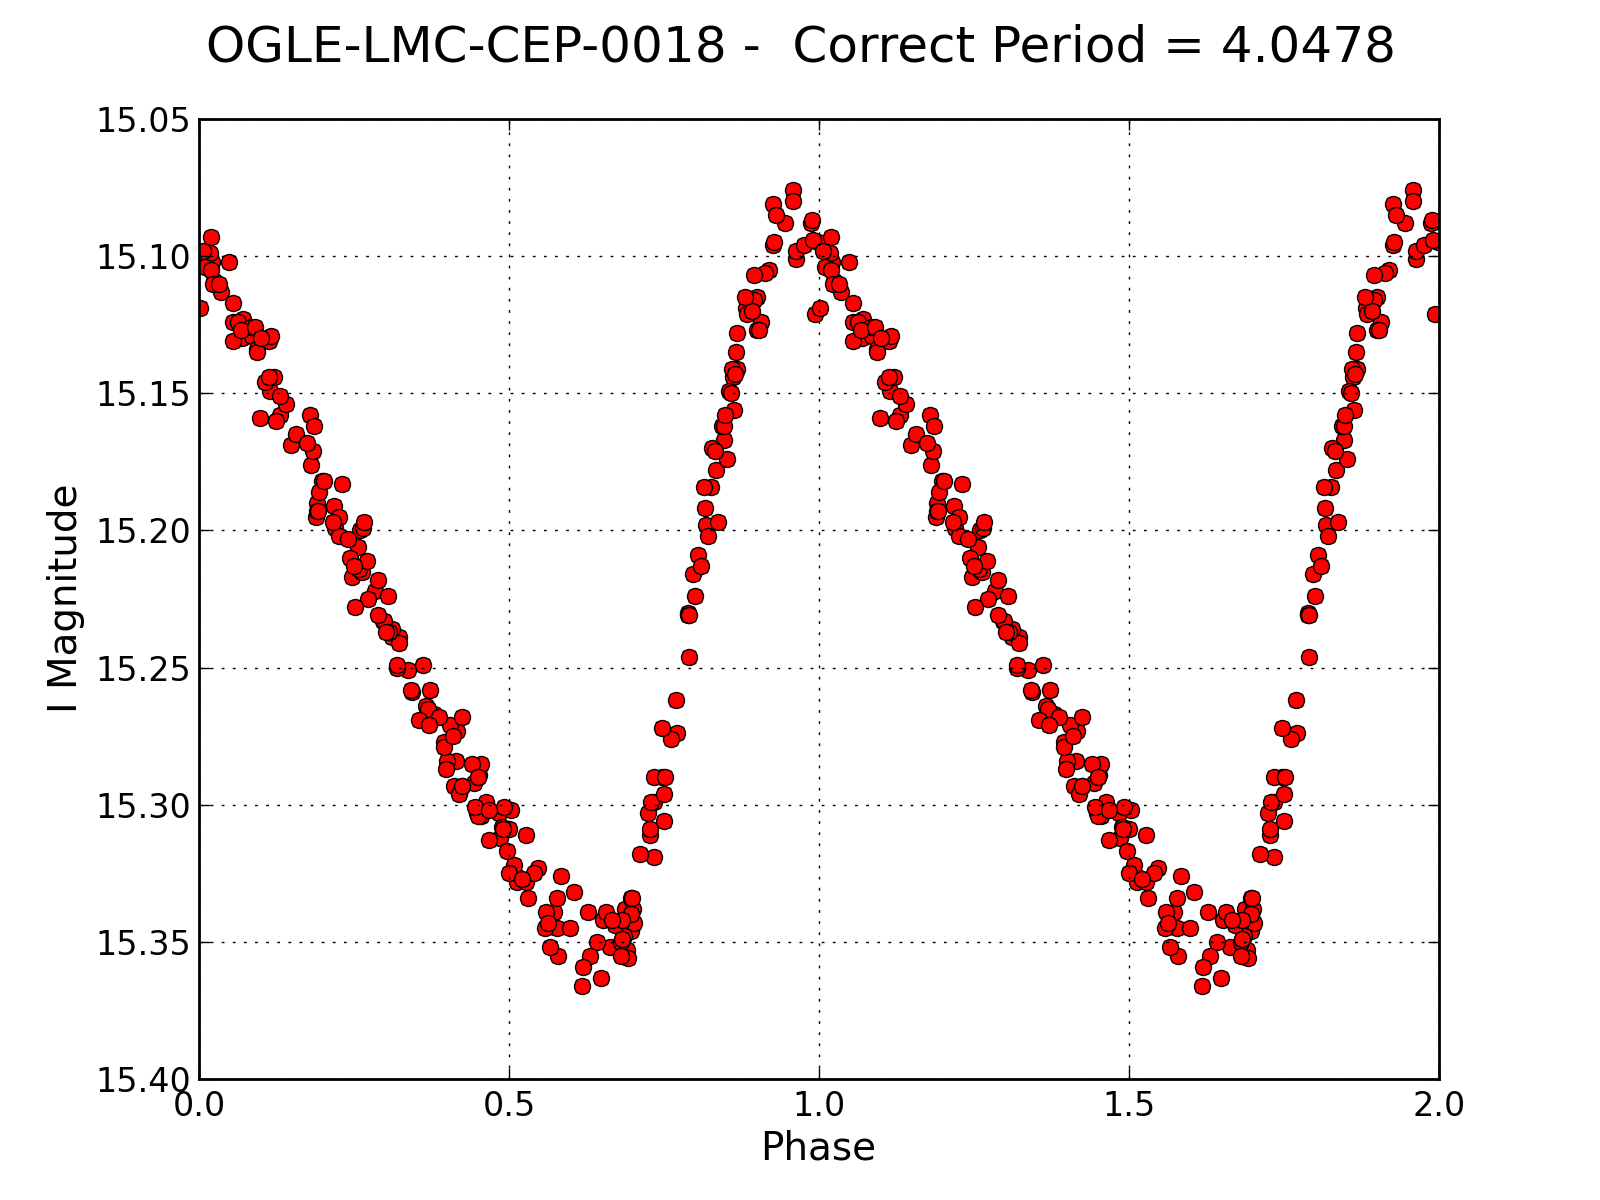
\includegraphics[width=\linewidth]{lightcurve_0018_correct_period.png}
%  \caption{Período correto}
%  \label{fig:right}
%\end{subfigure}%
%\begin{subfigure}{.5\textwidth}
%  \centering
%  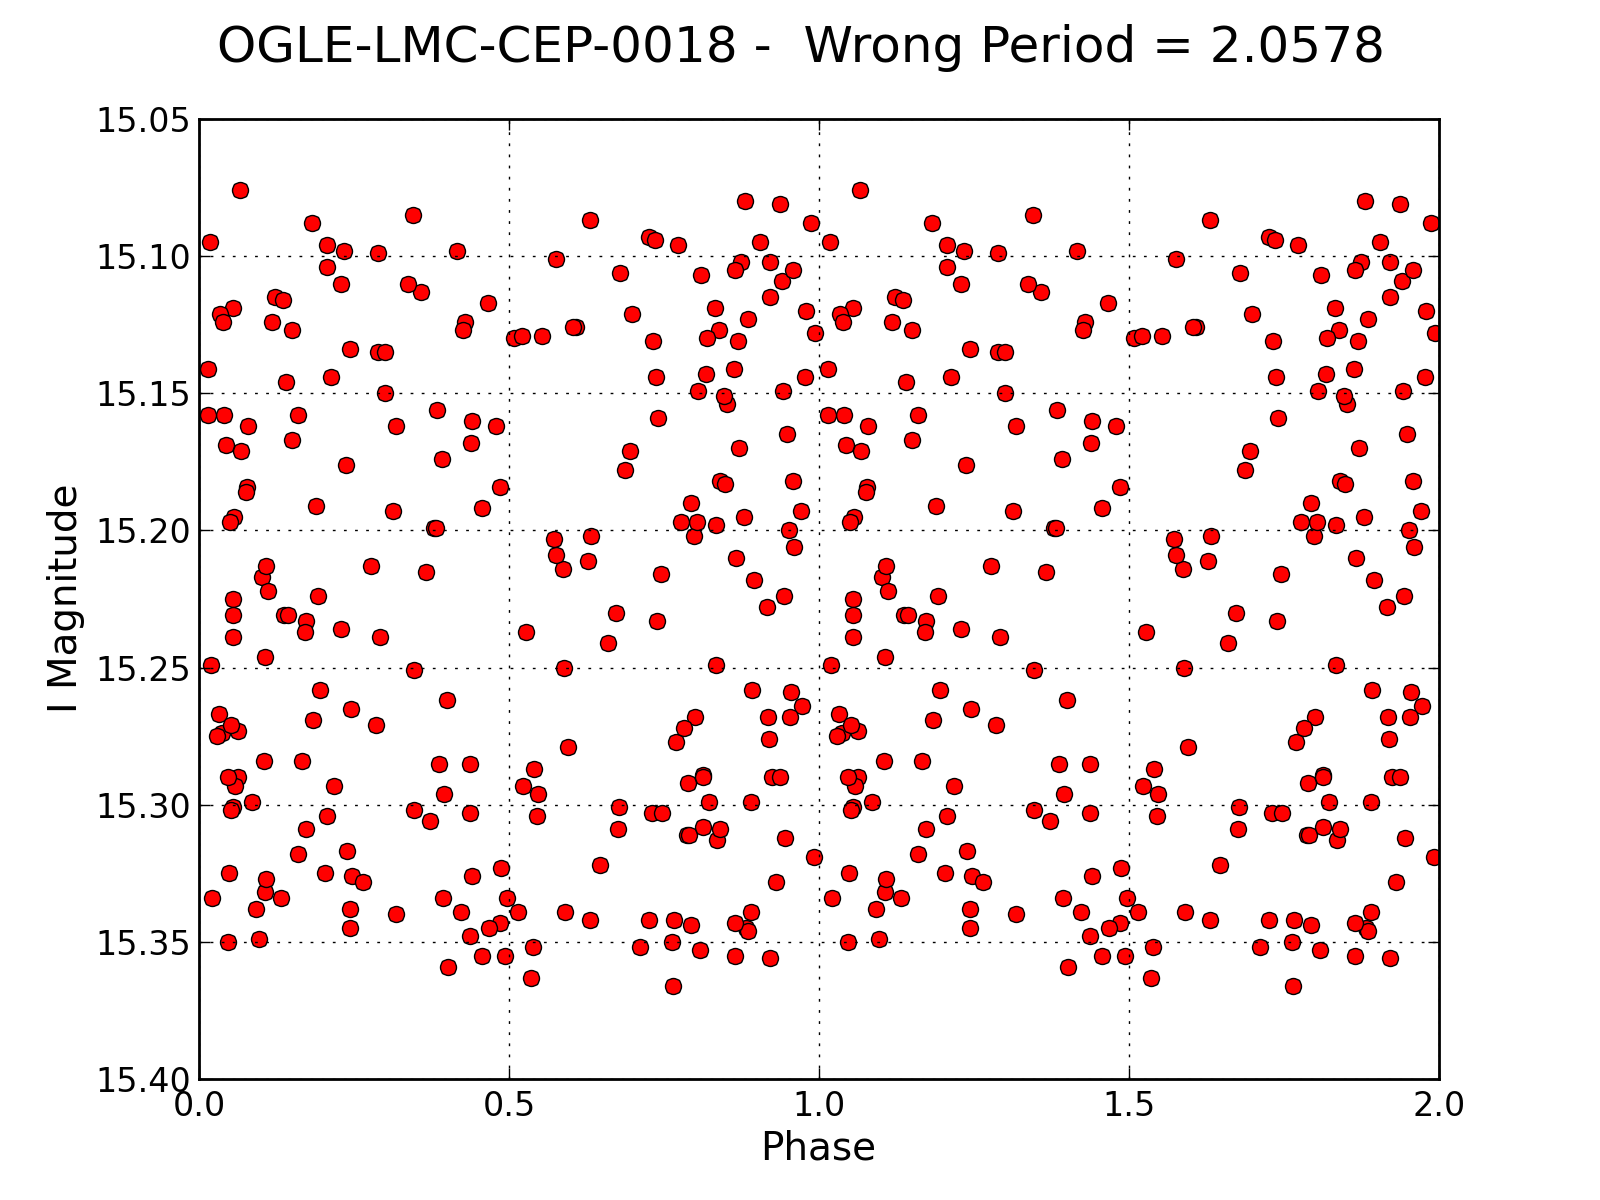
\includegraphics[width=\linewidth]{lightcurve_0018_wrong_period.png}
%  \caption{Período errado}
%  \label{fig:wrong}
%\end{subfigure}
%\caption{Exemplos de espa\c{c}o de fase}
%\label{fig:exemplo}
%\end{figure}
%
%Quando uma série temporal é dividida pelo período correto, será gerado uma dispersão com característica oscilante, como é o caso da figura \ref{fig:right}. Se o período utilizado na transforma\c{c}ão não for o correto, será gerado uma dispersão aleatória, sem forma definida, como mostra a figura \ref{fig:wrong}.
%
%\end{comment}

\section{Entropia de Shannon}

Na teoria de informação, a entropia ou entropia de Shannon \citep{informationTheory} é a medida de incerteza de uma variável. Em outras palavras, essa grandeza mede o grau de desordem para um sinal. Este sinal pode ser uma curva de luz ou até mesmo observações de velocidade radial de uma estrela \citep{entropy}. %A entropia de Shannon mede a falta de informação do nosso sistema, ou seja, quanto maior o seu valor mais incorreto a variável que estamos medindo. Desta forma, vamos procurar pela minimização da entropia no nosso espaço de fase.

O princípio deste método aplicado para a curva de luz de estrelas pulsantes se baseia na seguinte ideia: sendo sinais periódicos as curvas de luz das variáveis pulsantes, ao fazer a transformação para o espaço de fase, essa transformação com o período correto possui um certo grau de ordem, enquanto que a curva de luz construída com um período errôneo não possui ordem, gerando uma dispersão de pontos e todo o espaço de fase. Desta forma, a entropia de Shannon calculada para um sinal totalmente disperso em seu espaço de fase possui um valor maior do que essa mesma grandeza calculada para um sinal mais ordenado. Portanto, a entropia nos informa esse grau de desordem ou incerteza da variável em estudo, que neste caso é o período, e para um conjunto de períodos que queremos analisar a entropia de Shannon deve ser mínima para o período que produz a dispersão mais ordenada no espaço de fase. Um exemplo de espaço de fase com diferentes períodos é mostrado na figura \ref{fig:exemplo_entropia}.


\begin{figure}[!h]
\centering
\begin{subfigure}{.5\textwidth}
  \centering
  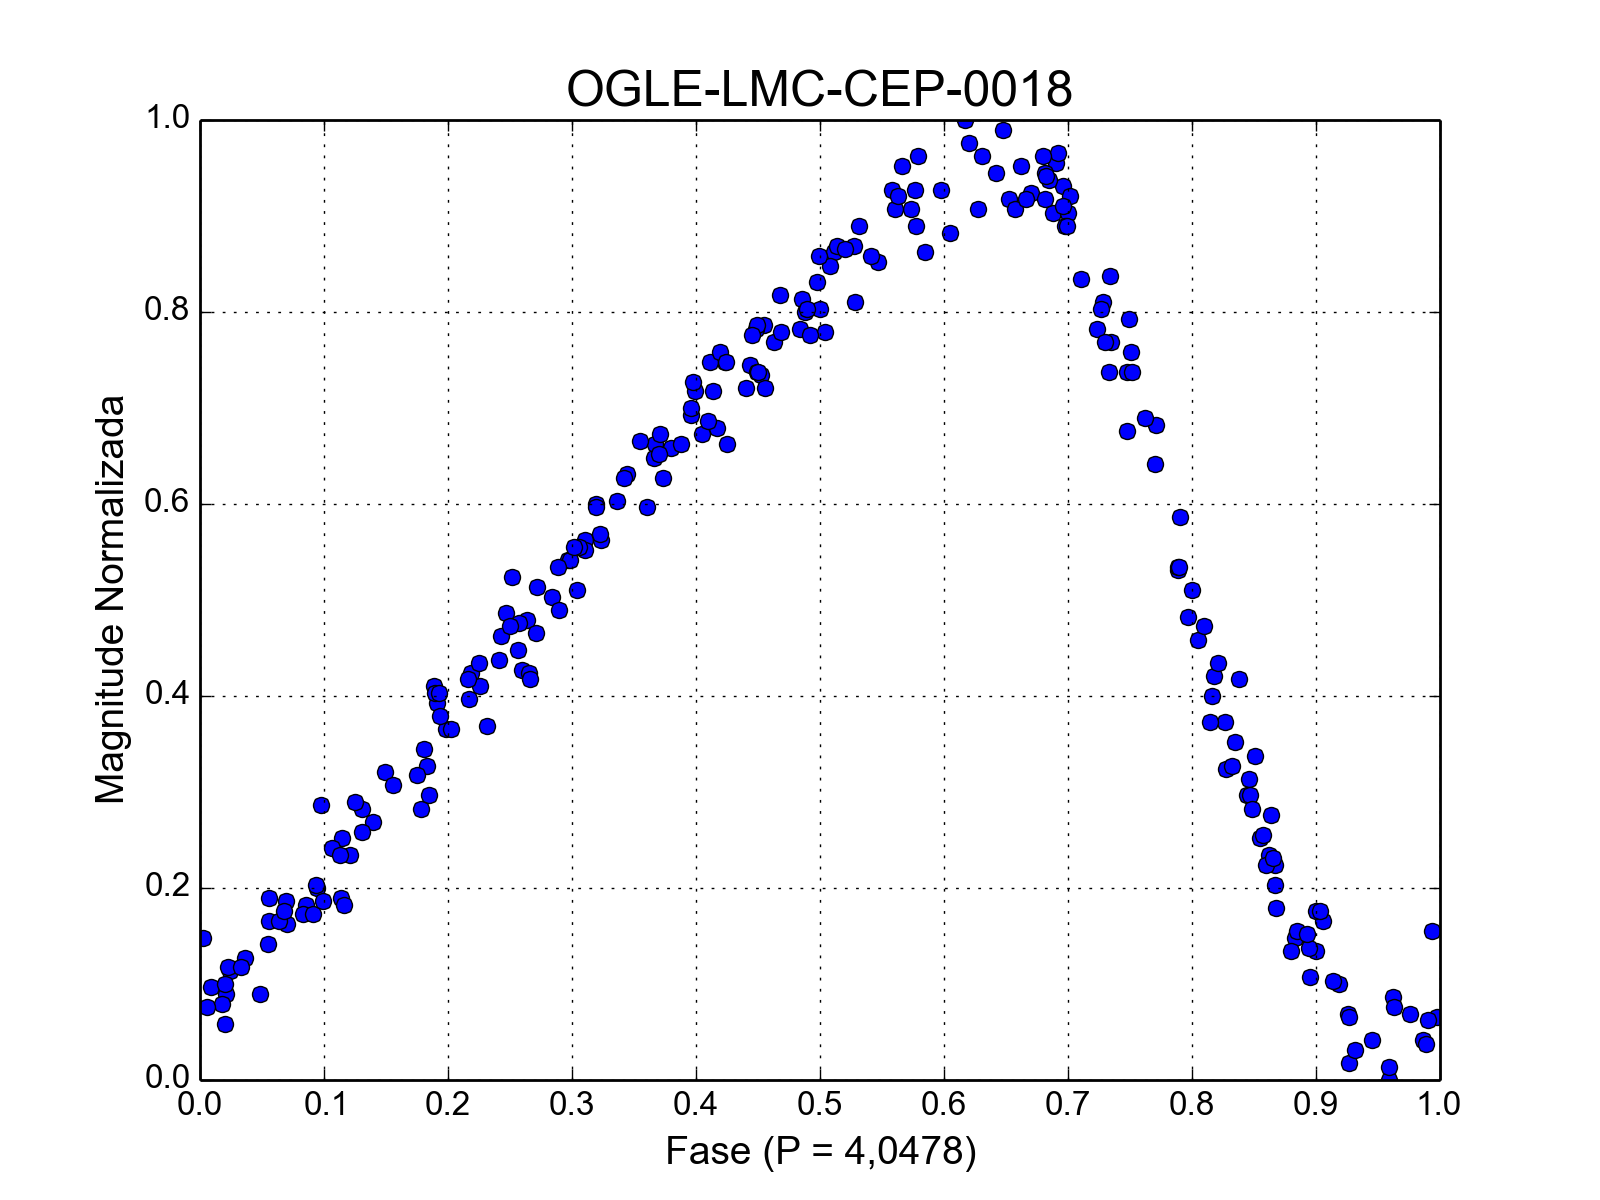
\includegraphics[width=\linewidth]{esp_fase_correto.png}
  \caption{Período correto}
  \label{fig:esp_fase_correto}
\end{subfigure}%
\begin{subfigure}{.5\textwidth}
  \centering
  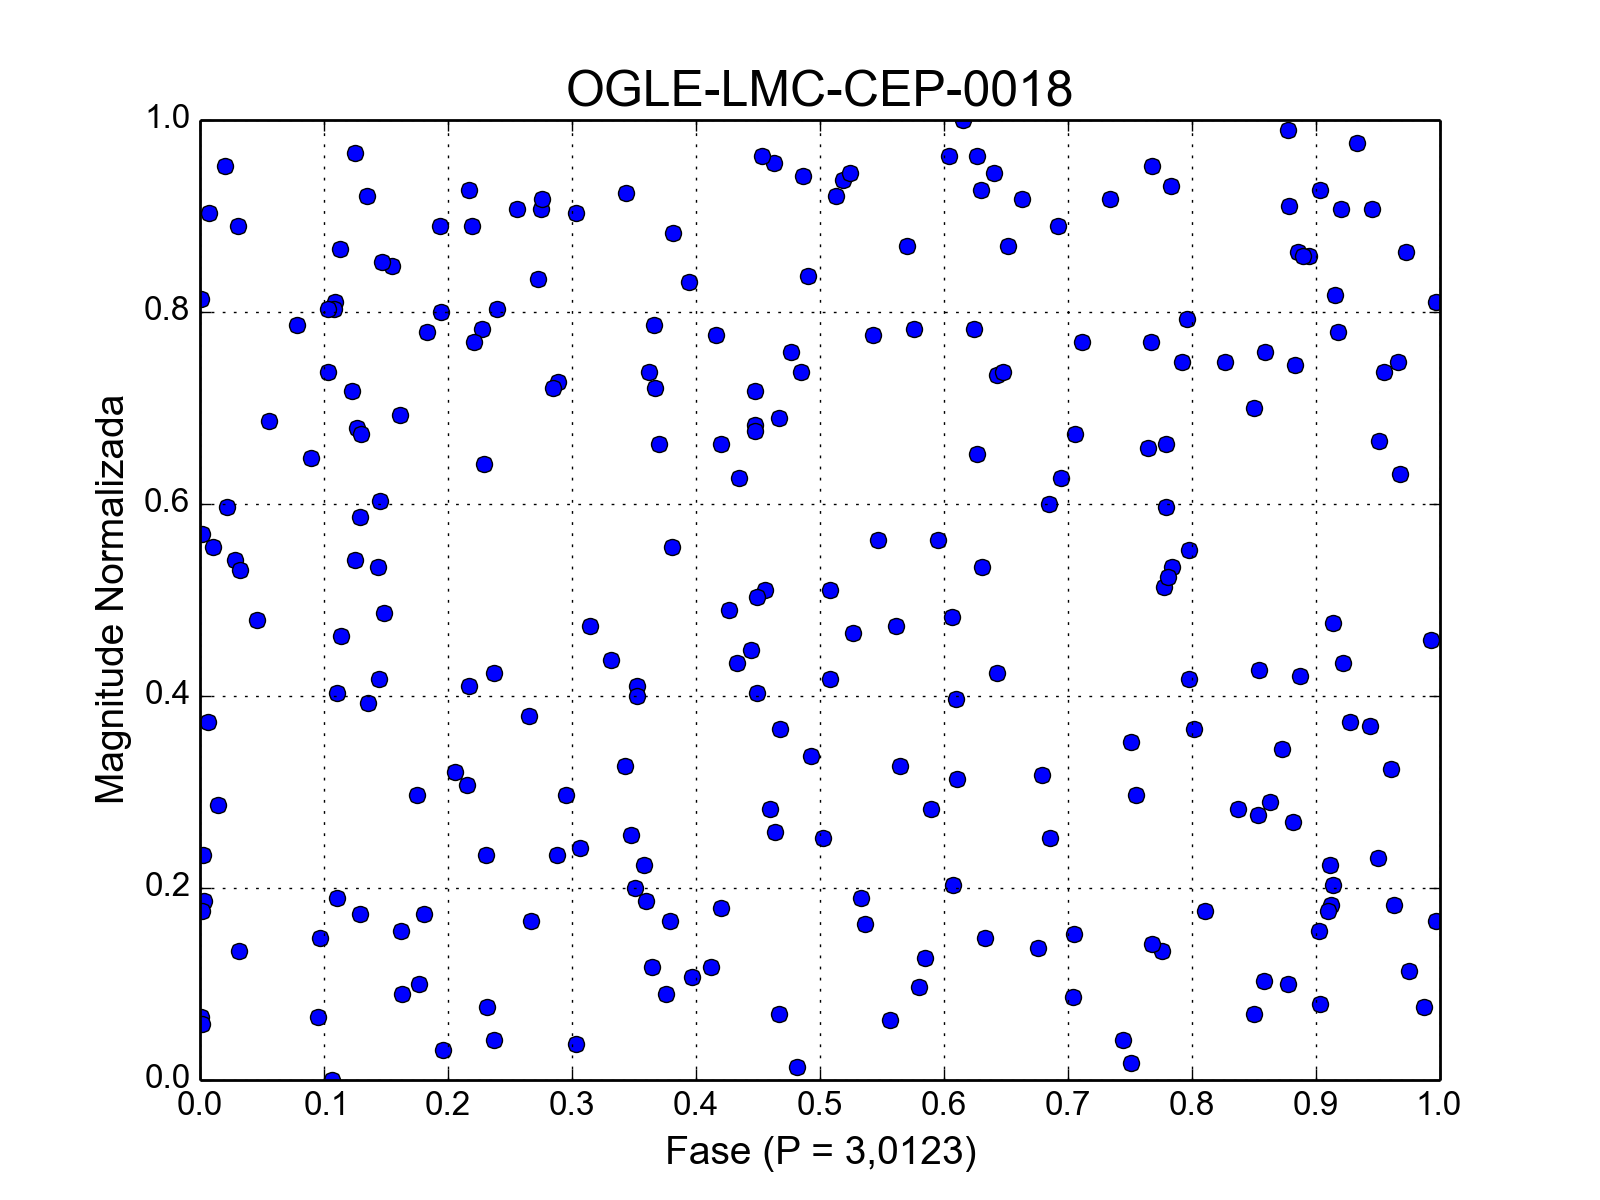
\includegraphics[width=\linewidth]{esp_fase_errado.png}
  \caption{Período errado}
  \label{fig:esp_fase_errado}
\end{subfigure}
\caption[Exemplos de entropia]{Exemplos da distribuição de pontos espaço de fase para a Cefeida OGLE-LMC-CEP-0018 do catálogo OGLE. O espaço de fase da imagem na esquerda foi construído utilizando o período correto ($P=4,0478$) e possui um valor para entropia de $H_c = 1,0762$. A imagem da direita foi utilizado um período aleatório ($P=3,0123$) e o valor de entropia calculado é $H_c = 1,5943$.}
\label{fig:exemplo_entropia}
\end{figure}


A entropia de Shannon foi aplicada pela primeira vez em curvas de luz por \citet{entropy}. Os autores normalizaram a magnitude das curvas de luz, transformaram para o espaço de fase e fizeram $m$ repartições nesse espaço. Desta forma, a entropia que é definida por:
\begin{align}
H = - \sum_i^m \mu_i \ln \mu_i
\end{align}
foi calculada. Nessa expressão, $\mu_i$ representa a probabilidade de ocupação da repartição $i$. Numericamente, a probabilidade de ocupação é calculada simplesmente contando os pontos de observação dentro da repartição e dividindo pela quantidade total de pontos. As vantagens desse método são a facilidade para lidar com sinais que possuam espaçamento variável entre os seu pontos, a simplicidade de aplicação e possui um embasamento matemático e estatístico bem definido dentro da teoria de informação, sendo que nem todos os métodos de detecção de períodos possuem esse ultimo item bem definido \citep{entropy}.


\subsection{Entropia condicional de Shannon }

A entropia de Shannon condicional surgiu da necessidade de contornar um problema bem conhecido da análise de curvas de luz: o efeito de \textit{Aliasing} causado pelo período $P=1$ dia. Este efeito ocorre devido as observações serem efetuadas sempre à noite, o que ocasiona um espaçamento de um dia entre os conjuntos de observação. A figura \ref{fig:periodo1dia} mostra a distribuição de pontos no espaço de fase normalizado utilizando o período $P=1$ dia. A entropia de Shannon calculada para uma distribuição desta forma retorna um valor pequeno, pois os pontos estão localizado em uma determinada parte do espaço.
\begin{figure}[!ht]
\centering
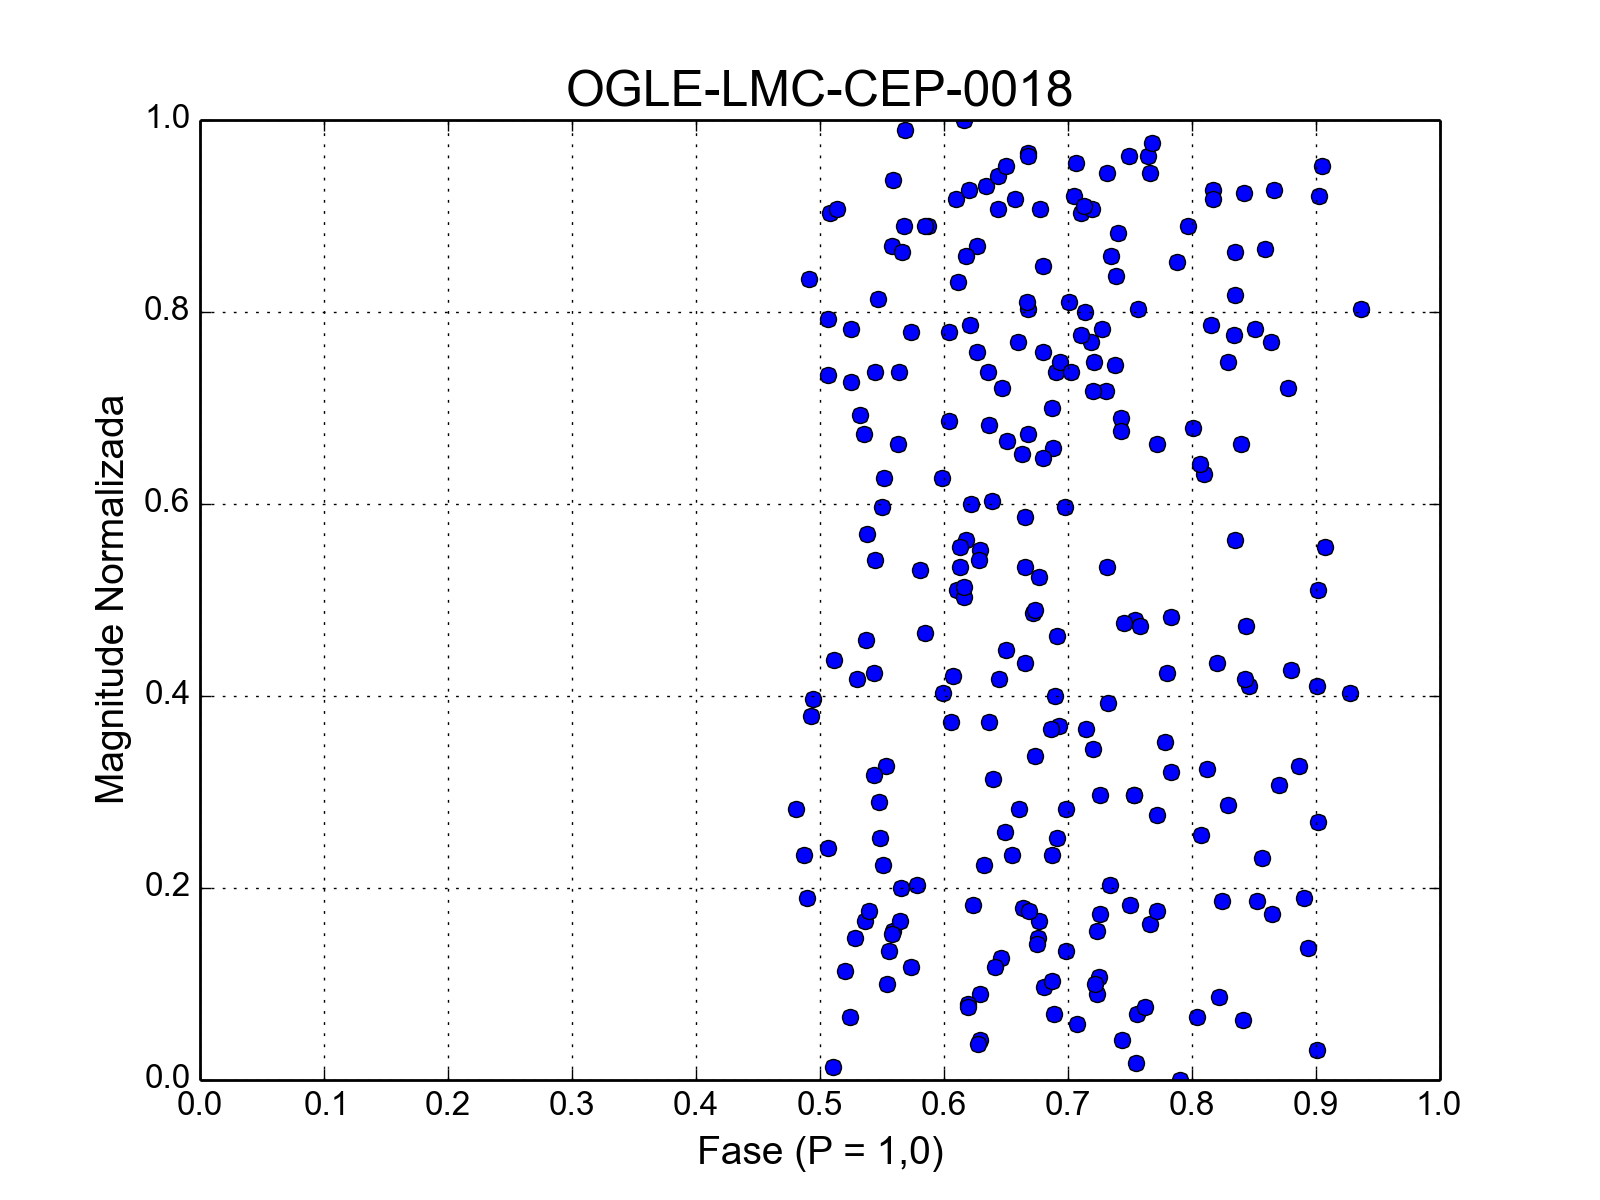
\includegraphics[width=0.5\linewidth]{esp_fase_1dia.png}
\caption[Efeito de \textit{Aliasing} com período de 1 dia.]{Efeito de \textit{Aliasing} devido ao período de 1 dia para a Cefeida OGLE-LMC-CEP-0018 do catálogo OGLE. Os pontos se localizam em uma determinada região do espaço de fase (menos da metade) o que faz com que a entropia calculada seja pequena. A entropia condicional foi proposta para lidar com este problema e para este caso o seu valor é $H_c=1,5542$.}
\label{fig:periodo1dia}
\end{figure}
Para lidar com esse problema, \citet{ce} propuseram a entropia de Shannon condicional. Nesta variação do método o espaço de fase é dividido em $i$ repartições na magnitude e $j$ repartições na fase e a entropia é calculada da seguinte forma:
\begin{align}
H_c = \sum_{i,j} p(m_i,\phi_j) \ln \left( \frac{p(\phi_j)}{p(m_i,\phi_j)} \right)
\end{align}
em que $p(m_i,\phi_j)$ é a probabilidade de ocupação na $i$-ésima repartição da magnitude e na $j$-ésima repartição da fase e $p(\phi_j)$ é a probabilidade de ocupação na $j$-ésima repartição da fase. Como estamos lidando com repartições retangulares:
\begin{align}
p(\phi_j) = \sum_i p(m_i,\phi_j)
\end{align}
ou seja, $p(\phi_j)$ é a soma das probabilidades na i-ésima coluna.

\citet{ce} analisaram o impacto no resultado da entropia causado pela quantidade de repartições e estimaram que $5$ repartições na magnitude ($\Delta m = 0,2$) e $10$ repartições na fase ($\Delta \phi = 0,1$) seriam ideais, pois quanto maior a quantidade dessas repartições mais recursos computacionais são necessários, e com essa escolha a entropia continua retornando bons resultados em pouco tempo.

Desta forma, a entropia de Shannon condicional será utilizada considerando $5$ repartições para a magnitude e $10$ para fase. Este método será aplicado para o espaço de fase normalizado para um conjunto de períodos que se quer analisar, calculando a entropia de Shannon condicional para cada espaço de fase criado para esse conjunto de períodos. O menor valor de entropia corresponde ao conjunto de pontos mais ordenado, o que seria o período correto da estrela \citep{ce} . Porém, antes de entrar em detalhes no algoritmo criado é necessário entender os dados utilizado no trabalho.


%\begin{comment}
%Quando uma estrela possui um comportamento periódico, a variação em sua magnitude é representada em ciclos iguais. Cada ciclo é uma fase. Se os ciclos são iguais, não importa qual ciclo nos estamos observando, apenas onde nos estamos no ciclo. Assim, o espaço de fase é uma representação de todos os ciclos observados em apenas uma fase, ou em apenas um ciclo. Assim, os pontos de sobrepõem e formam uma oscilação geral da estrela. Este espaço de fase é calculado pela seguinte expressão,
%\begin{equation}
%\phi_i = \frac{t_i}{P} - \Big[\frac{t_i}{P}\Big]
%\end{equation}
%em que $t_i$ é o i-ésimo dado do tempo, $P$ é o período de oscilação da magnitude e a quantidade entre colchetes representa apenas o numero inteiro da divisão.
%%Most of the entropy based methods are based on information entropy. In information theory, entropy is a measure of the uncertainty in a random variable. So, the entropy measures the lack of information of one variable.
%
%%Information theory based methods extract information from the probability density function and so include higher-order statistical moments present in the data whereas Fourier or analysis of variance techniques are based only on second-order statistical analyses. This implies that information theory brings better modeling of the underlying process and robustness to noise and outliers \citep{graB13}.
%
%
%%Para calcular a entropia condicional, primeiramente é necessário transformar os dados para o espa\c{c}o de fase e normalizar a luminosidade da estrela. Quando os dados são lidos pelo programa, ele gera dois vetores, um com os dados sobre o tempo e outro com os dados sobre a luminosidade da estrela. Para transformar o tempo em fase é necessário dividir cada um dos elementos do vetor tempo pelo período e subtrair o inteiro desta divisão,
%%\begin{equation}
%%\phi_i = \frac{t_i}{P} - \Big[\frac{t_i}{P}\Big]
%%\end{equation}
%%assim, temos um novo vetor com os dados da fase. O gráfico que pode ser obtido com os dados da fase e da luminosidade representa a dispersão da série temporal no espa\c{c}o de fase. A entropia condicional é calculada a partir desta dispersão.
%
%%Um exemplo de espa\c{c}o de fase é dado a seguir:
%
%\begin{figure}[h!]
%\centering
%\begin{subfigure}{.5\textwidth}
%  \centering
%  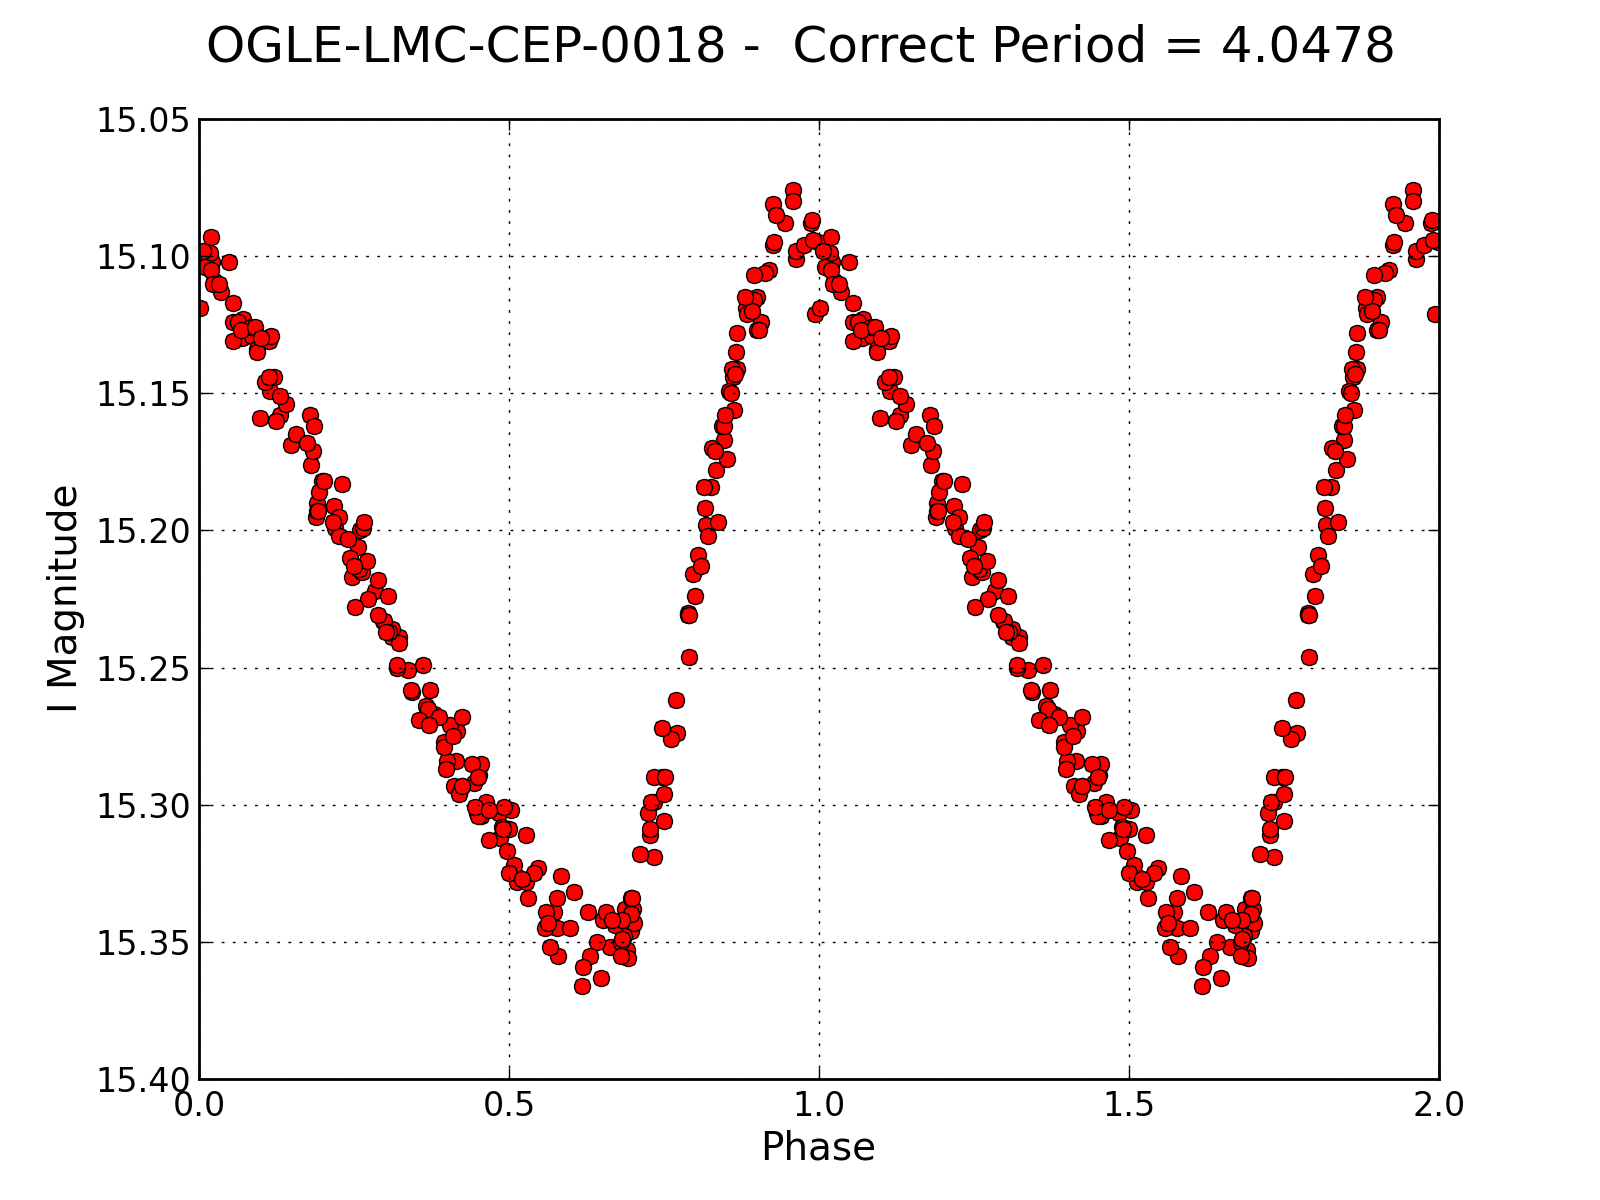
\includegraphics[width=\linewidth]{lightcurve_0018_correct_period.png}
%  \caption{Período correto}
%  \label{fig:right}
%\end{subfigure}%
%\begin{subfigure}{.5\textwidth}
%  \centering
%  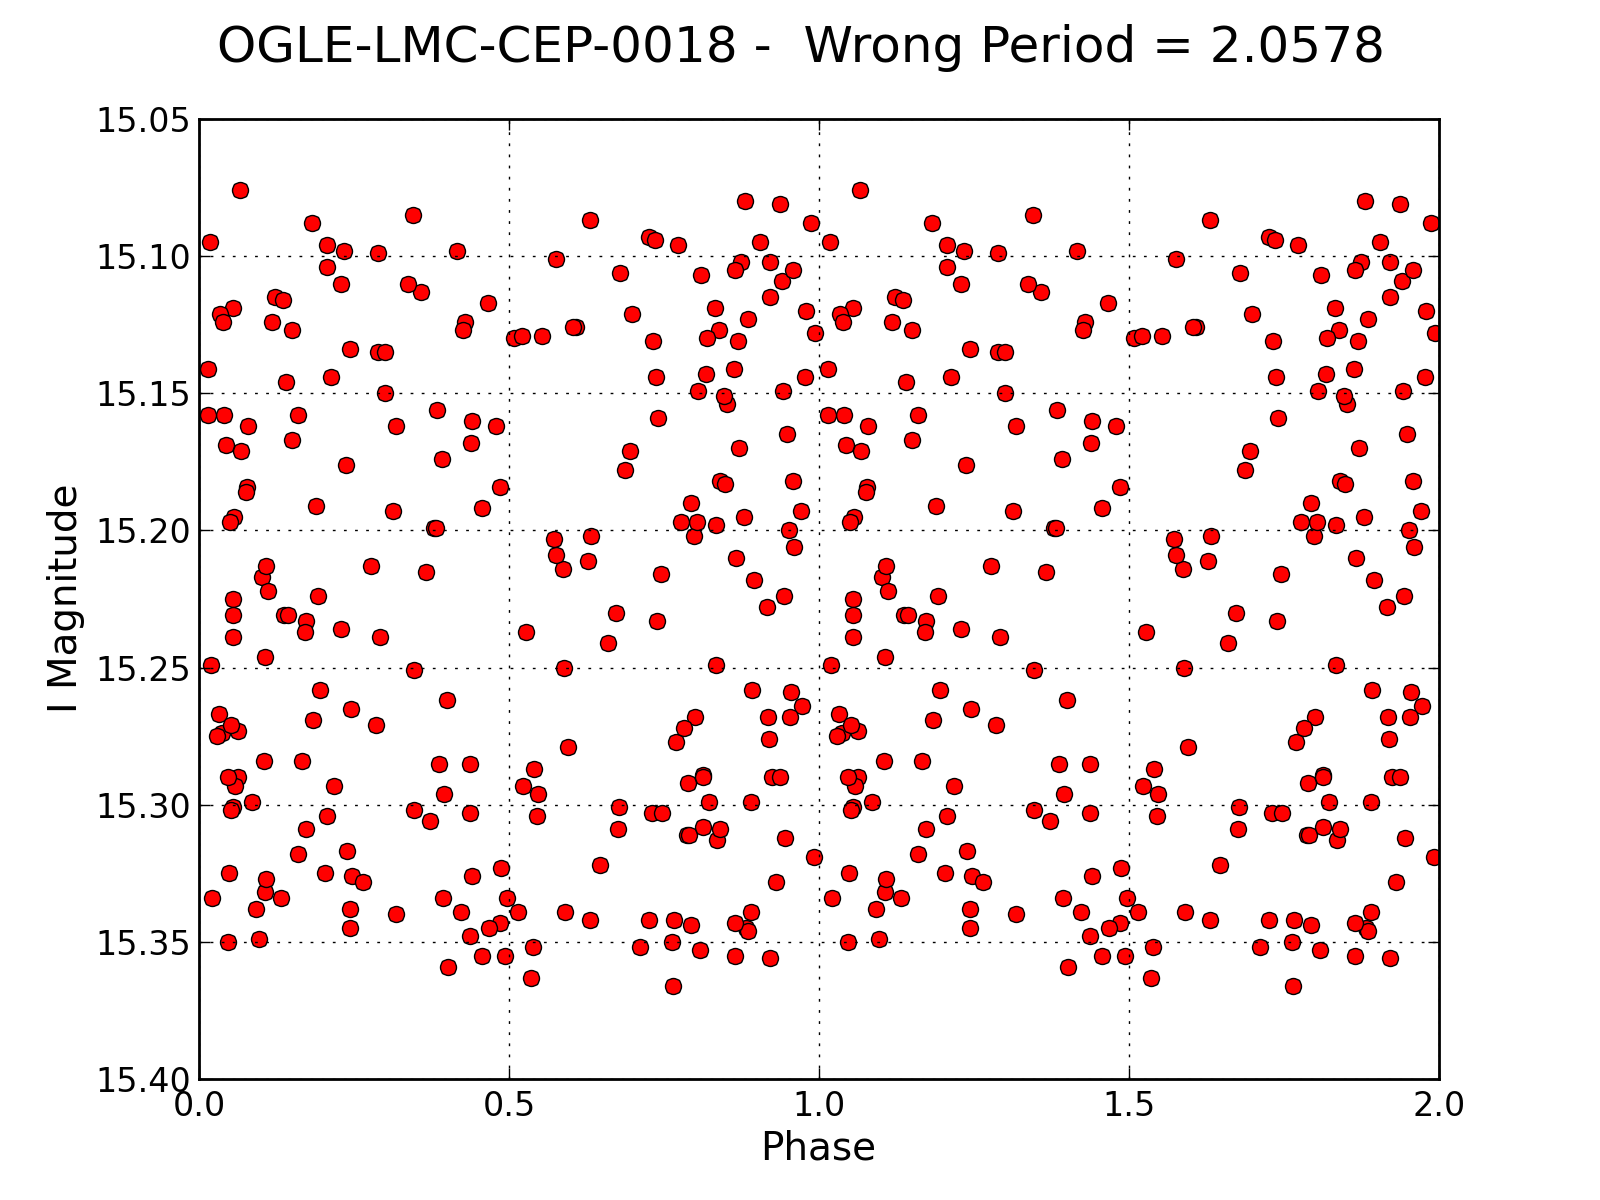
\includegraphics[width=\linewidth]{lightcurve_0018_wrong_period.png}
%  \caption{Período errado}
%  \label{fig:wrong}
%\end{subfigure}
%\caption{Exemplos de espa\c{c}o de fase}
%\label{fig:exemplo}
%\end{figure}
%
%Quando uma série temporal é dividida pelo período correto, será gerado uma dispersão com característica oscilante, como é o caso da figura \ref{fig:right}. Se o período utilizado na transforma\c{c}ão não for o correto, será gerado uma dispersão aleatória, sem forma definida, como mostra a figura \ref{fig:wrong}.
%
%\end{comment}

%Podemos observar que, no caso da figura \ref{fig:right}, os pontos se sobrepõem e formam uma curva. Assim, fazendo reparti\c{c}ões no dimensão da fase e da magnitude, podemos calcular a probabilidade dos pontos estarem localizados em cada um dos quadrados formados por estas reparti\c{c}ões em rela\c{c}ão a coluna em que eles estão e somá-los para obter uma grandeza. Esta grandeza é a entropia condicional, que é calculada pela seguinte formula \citep{ce},
%
%\begin{equation}
%H_c = \sum_{i,j} p(m_i,\phi_j)\ln \Big(\frac{p(\phi_j)}{p(m_i,\phi_j)}\Big)
%\end{equation}
%onde $p(m_i,\phi_j)$ é a probabilidade de ocupa\c{c}ão na $i$-ésima reparti\c{c}ão da magnitude e na $j$-ésima reparti\c{c}ão da fase e $p(\phi_j)$ é a probabilidade de ocupa\c{c}ão na $j$-ésima reparti\c{c}ão da fase. No caso de reparti\c{c}ões retangulares, %a probabilidade de ocupa\c{c}ão
%\begin{equation}
%p(\phi_j) = \sum_i p(m_i,\phi_j)
%\end{equation}

%A entropia de Shannon mede a falta de informa\c{c}ão do sistema, ou seja, quanto maior o seu valor, mais incorreto o período. Por isso que buscamos a minimiza\c{c}ão da entropia.
%Considerando estes dois exemplos, a probabilidade de de ocupa\c{c}ão das reparti\c{c}ões é menor na figura \ref{fig:right} do que na figura \ref{fig:wrong}. O menor valor de entropia condicional é associado ao período mais provável da estrela \citep{ce}.


\section{Catálogo OGLE}

O catálogo OGLE (\textit{The Optical Gravitational Lensing Experiment}) \citep{Udalski2008} consiste em 8 anos de dados observacionais cobrindo uma área de 40 graus quadrados na direção das Nuvens de Magalhães. Esse catálogo busca por estrelas variáveis tendo monitorado mais de 200 milhões de estrelas. As observações foram feitas utilizando os filtros Cousins I e V \citep{Cousins1973}. Na banda I, as observações possuem um tempo de $180 \si{s}$ de exposição tendo em média 400 medidas de observação. Por outro lado, a banda V possui em média apenas 30 medidas de observação. Os dados da sua terceira fase \citep{Udalski2008}, chamado de OGLE-III, são públicos\footnote{\url{http://ogledb.astrouw.edu.pl/~ogle/CVS/}} e foram utilizados nesse trabalho, dando prioridade para as observações na banda I devido a maior quantidade de medidas em relação a banda V.

Os dados de observação disponíveis são obtidos no formato .dat e possuem três colunas que significam tempo em dias Julianos, magnitude e erro na magnitude. Um exemplo de dado pode ser visto na tabela \ref{tab:dados}.

\begin{table}
\begin{center}
%\captionof{table}{Exemplo de dados}
\caption{Exemplo de dados do catálogo OGLE}
\begin{tabular}{c|c|c}
\toprule
Tempo & Magnitude & Erro \\
\midrule
2165,85271 & 15,130 & 0,007 \\
%\hline
2183,83450 & 15,326 & 0,008 \\
2238,62899 & 15,102 & 0,007 \\
$\vdots$ & $\vdots$ & $\vdots$ \\
\bottomrule
\end{tabular}
\label{tab:dados}
\end{center}
\end{table}

Nesse trabalho foram utilizados os dados de dois tipos de estrelas variáveis pulsantes localizadas na Grande Nuvem de Magalhães, as Cefeidas Clássicas e as RR Lyraes, sendo utilizados $3056$ Cefeidas classificadas entre modo fundamental (FU) e primeiro sobretom (FO) e $22651$ RR Lyraes também classificas entre modo fundamental (AB) e primeiro sobretom (C), totalizando $25707$ estrelas.

%We selected RRab stars from OGLE-III catalog that con- sists of 8-year archival data identified and characterized by the Fourier coefficients of the light curves (SZ09). The cat- alog contains 17, 693 RRab stars having a mean period of < Pab >= 0.576 days. The OGLE field in the LMC cov- ers nearly 40 deg2. Most of the observations were carried out using the Cousins I-band filter with exposure time of 180s having an average of 400 photometric observations. The catalog also contains V -band light curves of 17, 337 stars having an average of 30 data points per light curve. The



\section{Algoritmo}

Foi desenvolvido um algoritmo em \texttt{Python3} para calcular a entropia condicional de dados de estrelas variáveis pulsantes  pertencentes ao Catálogo OGLE-III. A figura \ref{alg:algoritmo} apresenta um pseudo-código do algoritmo. O código completo é apresentado no apêndice \ref{apend:algoritmo}. %\href{http://ogledb.astrouw.edu.pl/~ogle/CVS/}{Catálogo OGLE-III de estrelas variáveis}. %Os dados são obtidos no formato .dat e possuem três colunas que significam tempo, magnitude e erro. Um exemplo de arquivo pode ser visto na tabela \ref{tab:dados}.

\begin{algorithm}[!h]
\SetAlgoLined
\Entrada{Tempo e Magnitude \\
\Saida{Período $P$ que minimiza a entropia}
\Inicio{
Leitura dos dados de entrada como vetores; \\
Cria um vetor com $n$ períodos sendo P = ($p_1$ , $p_2$, $\cdots$, $p_n$); \\
Normalização da magnitude;\\
%\ParaCada{$p_i$ com $i = 1$  \Ate $i =n$}{
\ParaCada{$p_i$ em $P$}{
Transformar o tempo para o espaço de fase; \\
Faz as repartições e contabiliza os pontos; \\
Calcula a entropia de Shannon condicional; \\
Armazena a entropia calculada para o período $p_i$
}
Achar o valor mínimo de entropia: $E_{min}$ = min(Entropia) \\
Achar o período que minimiza a entropia:
$P_{E_{min}}$=P[min(entropia)]
}
\Retorna{$P_{E_{min}}$}
}
\caption[Pseudo-código do algoritmo.]{Pseudo-código do algoritmo em português estruturado.}
\label{alg:algoritmo}
\end{algorithm}

Para cada um dos dados das estrelas que serão analisadas, o programa faz a leitura das informações de tempo e magnitude da estrela, criando um vetor de períodos que serão analisados. Para uma Cefeida, esse vetor de períodos é criado com período inicial $p_1 = 0,1$ dias e período final $p_n = 32$ dias, com um intervalo entre os períodos de $0,001$ dia. Então, para cada um dos elementos do vetor período o algoritmo faz as seguintes ações: o tempo é transformado em fase, são feitas as repartições no espaço de fase e são contabilizados a quantidade de pontos em cada repartição; a entropia de Shannon condicional é calculada e o valor armazenado em um vetor entropia. % O mesmo é feito para o próximo período do vetor período até que sejam calculados a entropia para todos os dados deste vetor.
No fim, o algoritmo indica o menor valor do vetor entropia e qual período esta relacionado com este valor. %A figura \ref{fig:flow} apresenta um fluxograma do algoritmo.

%\begin{figure}[!hb]
%\centering
%	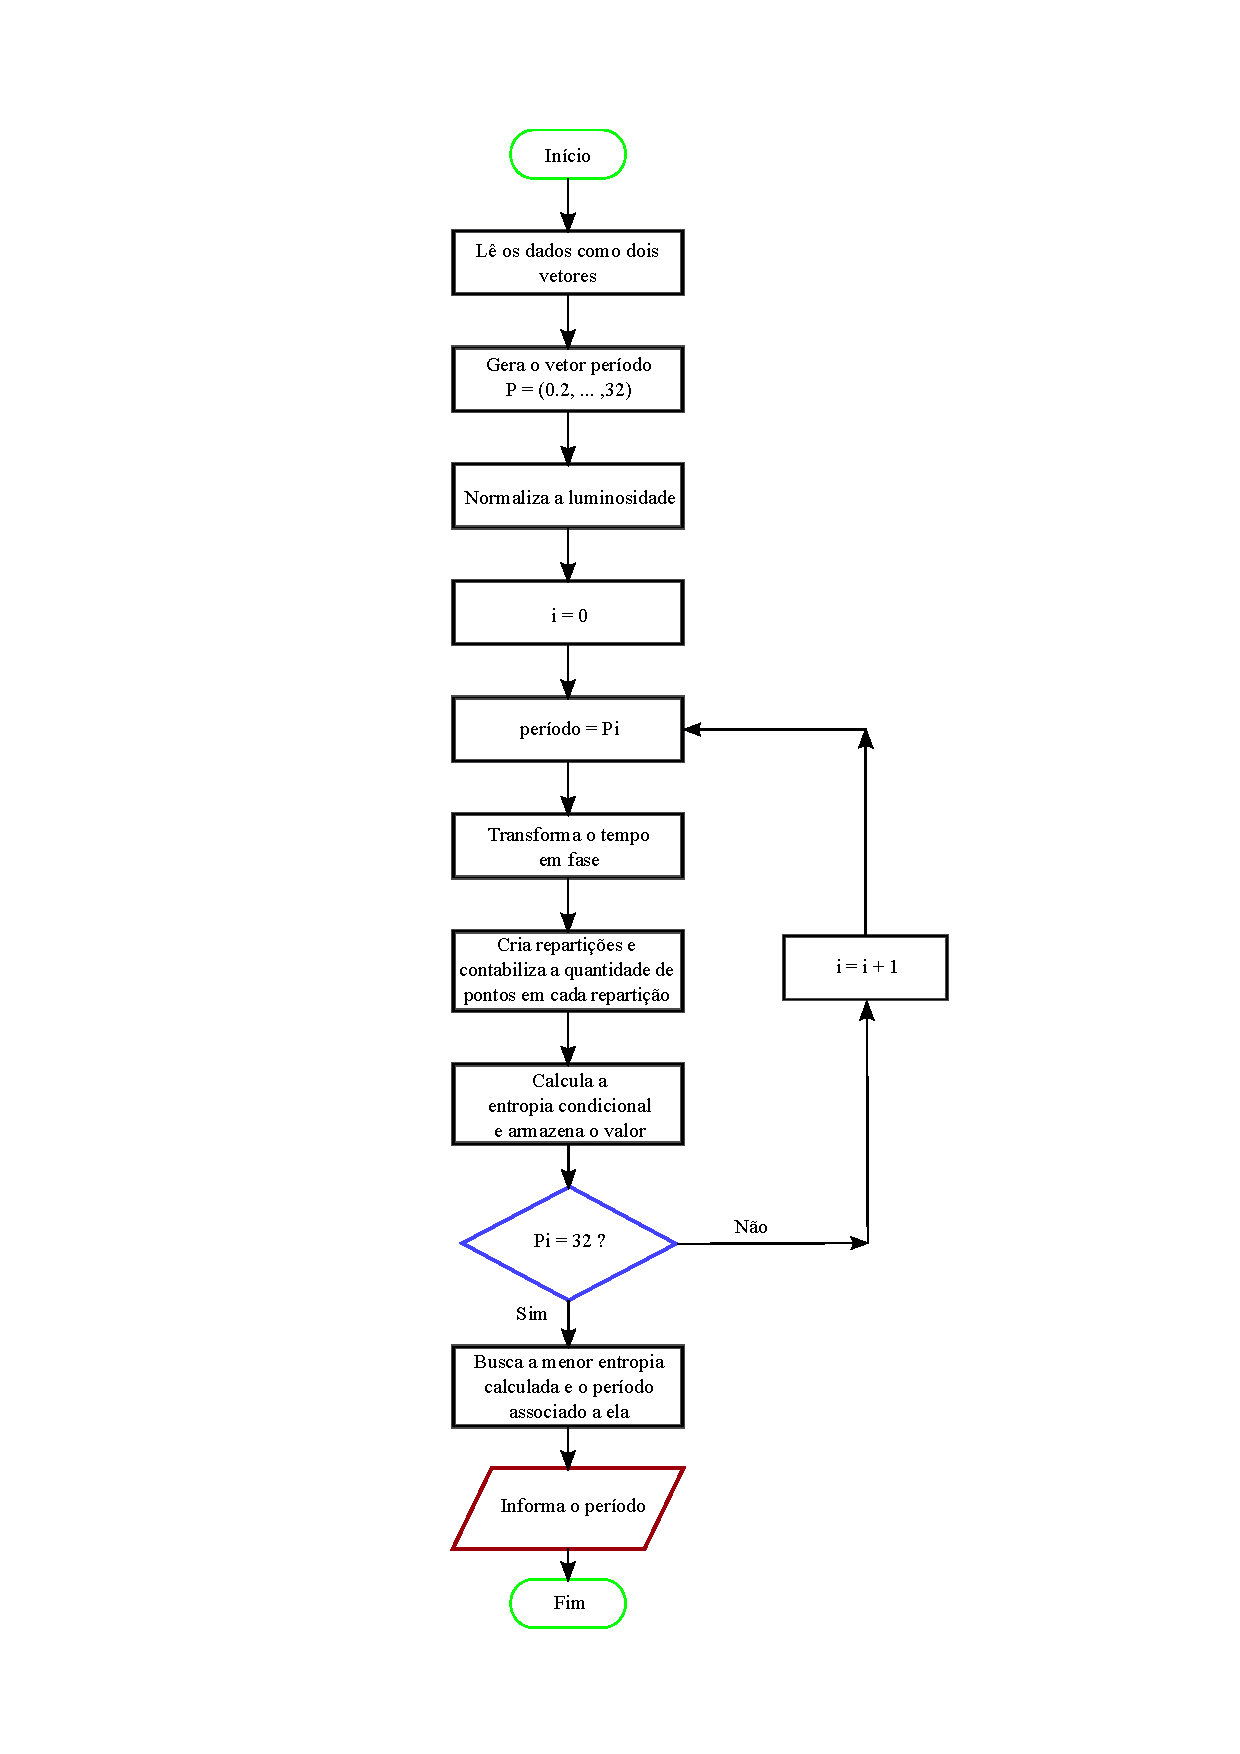
\includegraphics[scale=.6]{drawing.pdf}
%	\caption{Fluxograma do algoritmo}
%	\label{fig:flow}
%\end{figure}

\section{Análise Teórica}

Ao aplicar o algoritmo nos dados do catálogo podemos analisar como o método responde para dados reais. Porém, se quisermos analisar qual a abrangência de atuação desta técnica, é possível calcular a entropia de Shannon para um conjunto de dados teóricos em que seja conhecido o período. Desta forma, podemos entender como o formato de um sinal influencia nos resultados finais.

De acordo com %a literatura,
\citet{ce} e \citet{entropy}, um sinal periódico sintético que se assemelhe com os dados observacionais da maioria dos Surveys de estrelas variáveis pode ser construído utilizando a expressão:
\begin{align}
m(t) = A_0 + \sum_{i=1}^3 A_i \sin \left( \frac{2 k \pi t}{P} \right) + B \eta \label{eq:dado_sint}
\end{align}
Em que $m(t)$ é a magnitude sintética, $A_0$ é termo de deslocamento linear, os termos $A_i$ são termos de escala para as funções senos, $k$ é um parâmetro de escala para a amostragem do sinal, $t$ é o vetor tempo, $P$ é o período de oscilação do sinal, $\eta$ é uma distribuição gaussiana com média zero e desvio unitário que tem como função introduzir ruído no sinal e $B$ é um parâmetro de escala para esse ruído.

A amostragem ($f_s$) de um sinal representa a frequência de pontos de observação. Essa quantidade afeta diretamente a construção do vetor tempo, pois a amostragem é definida como:
\begin{align}
f_s = \frac{1}{dt} \quad \to \quad dt = \frac{1}{f_s} \label{eq:amostragem}
\end{align}
Ou seja, o intervalo de tempo depende do valor da amostragem. Desta forma, assim que for definida a nossa amostragem, podemos variar essa grandeza para construir os vetores tempos e com isso construir o sinal sintético para calcular a entropia de Shannon condicional e analisar os resultados. A análise de todos os dados, sintéticos e reais, será discutida no capítulo \ref{cap:resultados}.
